%----------------------------------------------------------------------------
%----------------------------------------------------------------------------
\frame
{
  \frametitle{Integraci\'on y Diferenciaci\'on Num\'ericas}
   
   \begin{itemize}
     \item<1-> Derivamos ajustando una recta a $n$ puntos consecutivos. La pendiente aproxima la derivada.
     \item<2-> Este m\'etodo tambi\'en suaviza los datos.
     \item<3-> Nunca tenemos $\frac{\Delta I}{\Delta V}=0$ porque $\Delta I>0$
     \item<4-> Tambi\'en tenemos que integrar
     \begin{equation*}\label{ins}
		I^{NS} = \frac{C^{NN}}{e} \int_{-\infty}^{\infty} dE\ \frac{|E|}{\sqrt{E^2-\Delta^2}} [f(E-eV)-f(E)]
	\end{equation*}
     \item<5-> Lo hacemos anal\'iticamente para $|E-\Delta|$ peque\~nos y numericamente para $|E-\Delta|\to\infty$
   \end{itemize}
  
}

%----------------------------------------------------------------------------
%----------------------------------------------------------------------------
\frame
{
  \frametitle{Diferencias al Modelo BCS}
  
      \begin{columns}
\begin{column}{0.6\textwidth}

  
  \begin{itemize}
  \item<1-> El modelo BCS no predice perfectamente la densidad de estados
  \item<2-> La causa puede ser que hay interaci\'on fon\'on-electr\'on adicional
  \item<3-> Giaever tambi\'en observ\'o este efecto
  \item<4-> Debido a esta diferencia no podemos ajustar los datos autom\'aticamente.
  \end{itemize}
    \end{column}
\begin{column}{0.4\textwidth}
	\begin{figure}[!h] \label{sample}
	\includegraphics<1-2>[width=\textwidth]{gv_theo_exp_7}
	\includegraphics<3->[width=\textwidth]{phonons_giaever}
	\end{figure}
\end{column}
 \end{columns} 


\uncover<5->{\textcolor{red}{\emph{Nos resignamos a hacerlo a mano\dots}}}
}

%----------------------------------------------------------------------------
%----------------------------------------------------------------------------
\frame
{
  \frametitle{Calculando Temperatura y Conductancia}
    \begin{columns}
\begin{column}{0.6\textwidth}
    \begin{itemize}
     \item<1-> Tenemos 3 par\'ametros independientes: $T$, $C_{NN}$ y $\Delta$ 
     \item<2-> Podemos hallar $T$ y $C_{NN}$ con otras medidas
     \item<3-> Calculamos $C_{NN}$ usando medidas de conductancia a $T\gg T_C$
     \item<4-> Calculamos $T$ con las medidas de presi\'on, y la curva de presi\'on de vapor del $He$.
  \end{itemize}
  
    \end{column}
    \begin{column}{0.4\textwidth}
	\begin{figure}[!h] \label{sample}
	\includegraphics<3>[width=\textwidth]{conductance2}
	\includegraphics<4>[width=\textwidth]{vap_he}
	\end{figure}
    \end{column}
    \end{columns} 

}

%----------------------------------------------------------------------------
%----------------------------------------------------------------------------
\frame
{
  \frametitle{Ajustando el Gap}
  
      \begin{itemize}
     \item<1-> Ahora podemos ajustar $\Delta$, el gap.
     \item<2->  $\Delta$ cambia poco ($0.1 meV$) en nuestro rango de temperaturas .
     \item<3-> Intentamos ajustar un valor de  $\Delta$ para todas medidas.
     \item<4-> Encontramos un valor de $\Delta = (1.4 \pm 0.1) meV$
     \end{itemize}
}


%----------------------------------------------------------------------------
%----------------------------------------------------------------------------
\frame
{
  \frametitle{Temperaturas mas bajas}
    \begin{columns}
\begin{column}{0.6\textwidth}
     \begin{itemize}
      \item<1-> Nuestra ultima medida tenia $T\approx 1.2K$
      \item<2-> Hemos encontrado una curva de conductancia muy distincta.
      \item<3-> Se puede explicar con la transicion de partes del $Al$ a superconductancia.
      \item<4-> No hay conductancia negativa, asi que no esta totalmente superconductor.
     \end{itemize}
     
       \end{column}
\begin{column}{0.4\textwidth}
	\begin{figure}[!h] \label{sample}
	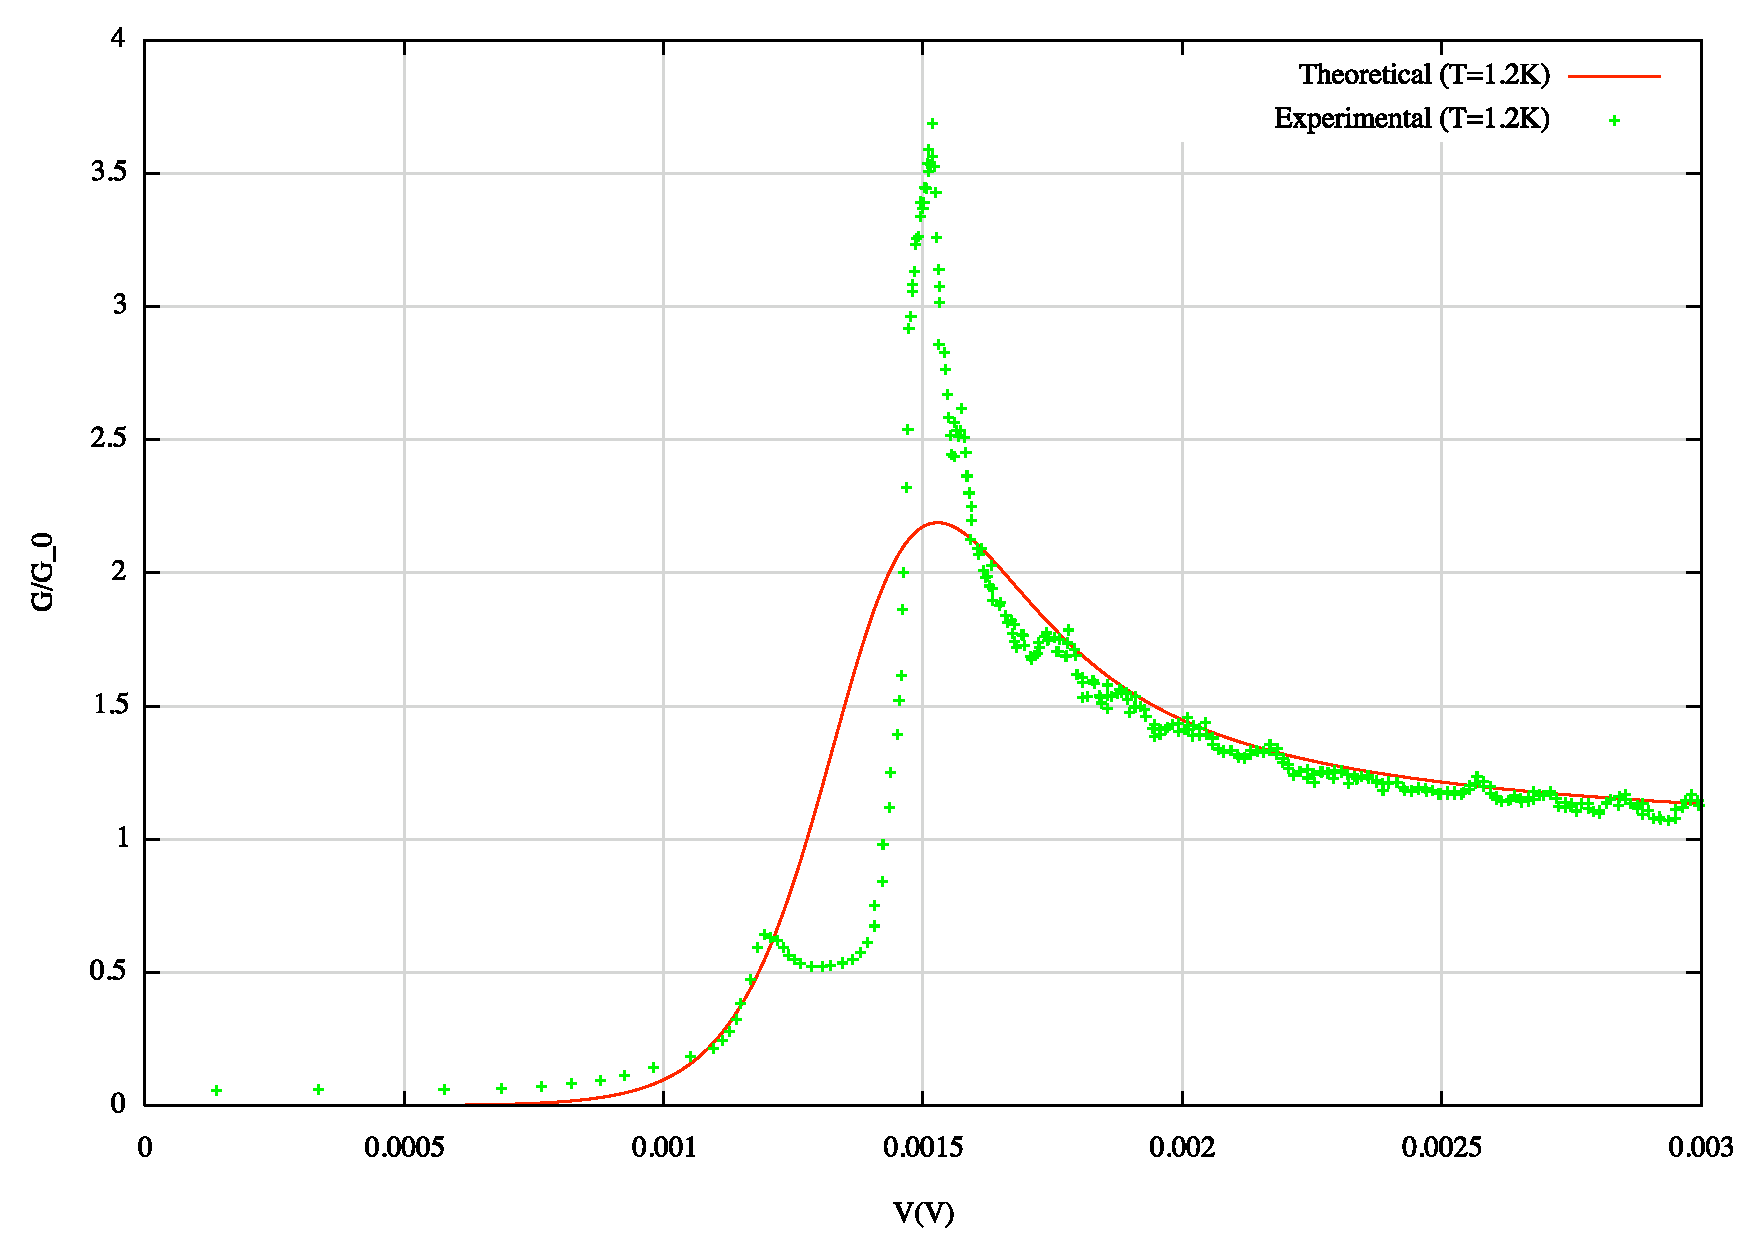
\includegraphics[width=\textwidth]{gv_theo_exp_10}
	\end{figure}
\end{column}
\end{columns} 

 }
 %----------------------------------------------------------------------------
%----------------------------------------------------------------------------

